\chapter{Introduction} \label{chapt:Introduction}

A change in distribution of a machine learning environment is known as concept drift. Due to the ubiquity of change, concept drift is an endemic problem in machine learning and data science, and practitioners should always be aware that their models may degrade over time as a result. Unless concept drift can be ruled out {\it a priori}, practical machine learning systems will generally need a strategy for adapting to a changing environment.

Over the last few decades, a considerable amount of research has been dedicated to detecting and adapting to concept drift \cite{gama_survey}\cite{barros_comparison}. Because concept drift is such a broad category of phenomenon, this research has necessarily had to focus on a specific formulation of concept drift. This formulation is roughly
\begin{displayquote}
  At regular time intervals, new instances become available. A learner must thereupon predict the label corresponding to the new instance. Immediately after the model has made the prediction, the true label becomes available. The learner then incrementally learns from the new instance-label pair in an online manner.
\end{displayquote}
We will call this the {\bf standard formulation of the concept drift problem}, or simply the standard formulation. A common variant of the standard formulation is that instances and labels become available in batches rather than individually. Practically, this often makes little difference. The standard formulation is attractive from an academic perspective. It is simple and covers a wide class of problems. It is easily rendered in synthetic benchmark datasets against which progress in the field can be measured. It can be naturally expressed in formal mathematics, so is easily tractable to theoretical study.

There are broadly two approaches to handling concept drift. ``Blind" approaches do not explicitly model drift, instead allowing the model to gradually adapt to the new environment. ``Informed" approaches, instead employ {\bf drift detectors} to explicitly detect when concept drift has occurred so that the model can be retrained \cite{gama_survey}. Blind approaches are often inadequate, as it can take too long for the model to adapt to the new environment. Informed approaches work roughly as follows:
\begin{displayquote}
  The drift detector monitors some performance metrics of the model. When it detects a degradation in performance, it makes a ``guess" about when the drift occurred, and automatically retrains the model using data from that drift point.
\end{displayquote}
We will call this the {\bf standard approach to concept drift adaptation}, and it is illustrated in Figure \ref{fig:standard_adaptation}.

\begin{figure}
    \centering
    
    % Define block styles
    \tikzstyle{decision} = [diamond, draw, fill=blue!20, 
        text width=4.5em, text badly centered, node distance=3cm, inner sep=0pt]
    \tikzstyle{block} = [rectangle, draw, fill=blue!20, 
        text width=5em, text centered, rounded corners, minimum height=4em]
    \tikzstyle{line} = [draw, -latex']
    \tikzstyle{cloud} = [draw, ellipse,fill=red!20, node distance=3cm,
        minimum height=2em]
    
    % Define block styles
    \begin{tikzpicture}[node distance = 2cm, auto]
        % Place nodes
        \node (start) {};
        \node [block, right of=start, node distance=3cm] (model) {Model};
        \node [block, right of=model, node distance=6cm] (detector) {Detector};
        \node [right of=model, distance=3cm] (mid) {};
        \node [cloud, below right of=model, align=center, node distance=4cm] (action) {retrain};
        % Draw edges
        \path [line] (start) -- node {data}(model);
        \path [line] (model) -- node {error rate}(detector);
        \path [line] (detector) |- node {drift detected} (action) -| (model);
        % \path [line] (action) ;
    \end{tikzpicture}
    \caption{Informed approach to concept drift adaptation.}
    \label{fig:standard_adaptation}
\end{figure}

\section{Motivation}

In many applications the standard formulation of the concept drift problem diverges from reality in important ways. In some cases this may only mean that existing drift detectors are theoretically inappropriate, but practically serviceable. In other cases it may be a fatal flaw that renders drift detectors unusable.

Our exploration of the practical application of concept drift detection is motivated by a concrete problem from medical data science. We will return to this motivating example throughout the thesis to illustrate procedures, inform intuitions, and justify decisions. The problem is detecting concept drift for a GP referrals triage decision support:
\begin{displayquote}
  When a patient is referred to a medical facility, the referral is documented with free text and structured data, containing such information as condition, comorbidities, and demographics. From this data a clinician will make a decision about how urgently the patient needs to be addressed, and assign the patient a triage priority label. Some examples of triaging manuals are publicly available \cite{aus_triage}\cite{UK_mental_triage}\cite{musculoskeletal_services}.

  Referral documents are often electronic, reflecting a broad trend of medical facilities switching from paper documents to electronic health records (EHR) \cite{ehr_adoption}. These electronic documents present an opportunity \cite{ehr_opportunities}: supervised learning can train a model to predict triage labels for referral documents. This model can then be incorporated into a decision support system to help clinicians make more efficient and systematic triage decisions.

  An obvious benefit of such a support system is guaranteeing that all referrals can be triaged in a timely manner. Automatic support system triage can provide a first pass on referrals, which can then be manually reviewed by clinicians once they are available. Another area in which this decision support system is expected to benefit public health is by countering potential bias in the healthcare system. Due to inefficient triaging, vulnerable ethnic groups are susceptible to being ``bumped down the queue" by those less in need \cite{pdh}.

  Staff, resources, policy, and best practices evolve over time in medical environments, so it is important that a decision support system is able to detect and adapt to these changes. Suppose one demographic group is discovered to be particularly susceptible to some condition. Clinicians may respond by giving this demographic systematically higher priority. A decision support system must be able to promptly detect that such a change has occurred, and trigger appropriate actions for the model to be corrected. That is, a decision support system must be sensitive to {\it concept drift}.

  The proposed method for handling concept drift is illustrated in Figure \ref{fig:referrals_triage}. When a GP makes a referral, it is sent to the model, a clinician, and a drift detector. The model predicts the triage label for the referral, and this prediction is sent to both the clinician, for decision support, and the drift detector. When the clinician eventually arrives at an ``official" triage label, this is also sent to the drift detector. Based on these inputs, if the drift detector ever detects concept drift, it notifies a data scientist and provides details of the drift. The data scientist then decides if the model is still fit for purpose (FFP) after this concept drift. If not, the data scientist may decide to retrain the model, or recall the model if its performance cannot be recovered to an acceptable level.

  If the model is to be retrained, the data scientist must decide what data can be included in the new training set, based on the information provided by the drift detector. For example, if the distribution of labels for referrals for condition $X$ changed one month ago, then a good choice of training data may be referrals from the last month for condition $X$, but the full dataset for all other conditions.
\end{displayquote}

\begin{figure}
    \centering
    \tikzstyle{block} = [rectangle, draw, 
        text width=5em, text centered, rounded corners, minimum height=6em] % fill=blue!20, 
    \tikzstyle{line} = [draw, -latex']
    \tikzstyle{cloud} = [draw, ellipse,fill=yellow!20, node distance=3cm,
        minimum height=3em]
    
    \begin{tikzpicture}[node distance = 3cm, auto]
        % Place nodes
        \node [block] (gp) {
\includegraphics[width=1cm]{images/referrals_triage/gp.png}\\GP};
        \node [cloud, right of=gp] (referral) {Referral};
        \node [cloud, above right of=referral, align=center] (support) {Decision\\support};
        \node [block, above of=support] (model) {
\includegraphics[width=1cm]{images/referrals_triage/model.png}\\Model};
        \node [block, below of=support, node distance=5cm] (clinician) {
\includegraphics[width=1cm]{images/referrals_triage/clinician.png}\\Clinician};
        \node [cloud, right of=clinician, node distance=4cm, align=center] (label) {Triage\\label};
        \node [cloud, right of=model, node distance=4cm] (prediction) {Prediction};
        \node [block, right of=referral, node distance=6cm] (detector) {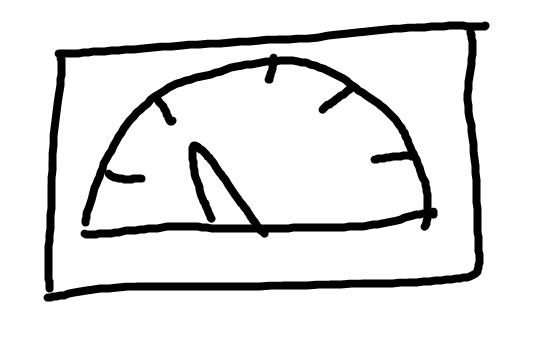
\includegraphics[width=1cm]{images/referrals_triage/detector.png}\\Detector};
        \node [cloud, above of=model] (retrain) {Retrain};
        \node [cloud, right of=detector, align=center] (detection) {Drift\\detection};
        \node [block, above of=retrain] (ds) {
\includegraphics[width=1cm]{images/referrals_triage/datascientist.png}\\Data scientist};
        % Draw edges
        \path [line] (gp) -- (referral) -- (detector);
        \path [line] (referral) |- (clinician);
        \path [line] (clinician) -- (label) -- (detector);
        \path [line] (referral) |- (model);
        % \path [line] (referral) -- (detector);
        \path [line] (model) -- (prediction) -- (detector);
        \path [line] (detector) -- (detection) |- (ds);
        \path [line] (ds) -- (retrain);
        \path [line] (retrain) -- (model);
        \path [line, dashed] (model) -- (support) -- (clinician);
    \end{tikzpicture}
    \caption{The proposed method for handling concept drift in GP referrals triage.}
    \label{fig:referrals_triage}
\end{figure}

This setting diverges from the standard concept drift problem formulation in that:
\begin{itemize}
  \item In the standard formulation labels become available immediately after prediction. In the GP referrals context, there may be an arbitrarily long delay between the model predicting a triage label for a given referral and a clinician providing a correct triage label. Furthermore, the labels may become available in a different order to the referrals.
\end{itemize}
This setting also diverges from the standard approach to concept drift adaptation in that:
\begin{itemize}
  \item In the standard appraoch, the detector automatically guesses when drift occurred and retrains the model based on that guess. In the GP referrals context, there is a human in the loop (the data scientist) who can make informed decisions about whether the detector requires retraining or recall, and about what training data to use if it does require retraining.
\end{itemize}

In order to make an informed decision about what action to take, the data scientist will want to know:
\begin{itemize}
  \item Has the distribution of referrals changed? And if so, does this require model retraining or recall? Can this be detected before all the labels have arrived, which could take arbitrarily long?
  \item Will retraining the model on more recent data actually improve its performance? Or is performance irreparably degraded under the new distribution because the referral tasks have become intrinsically more difficult?
  \item How severe was the concept drift and how long ago did it occur? Can the uncertainty on these questions be quantified?
\end{itemize}
Existing drift detector methods are unable to provide this information. This is the problem we intend to solve in this thesis.

\section{Problem Statement}

We are interested in applying concept drift detection to a task where instances and labels arrive in an irregular manner, and where model retraining is facilitated by a human expert. The main research questions we explore are:
\begin{enumerate}
  \item How can we get early warnings that a machine learning model is no longer fit for purpose? Specifically, if labels have delayed arrivals, then how can we get an early warning that the distribution of features has changed?
  \item How can we differentiate between reducible and irreducible error from concept drift?
  \item How can we quantify the uncertainty around drift timing and its severity?
\end{enumerate}

\section{Objectives}

The aims of our research are:
\begin{enumerate}
  \item To develop a system for providing early warnings that a model requires retraining or is no longer fit for purpose? Specifically in cases where instance and label values become available in an irregular manner?
  \item To develop drift detection algorithms which is only triggered by irreducible, rather than reducible error.
  \item To develop a drift detection method which quantifies the uncertainty around drift timing and its severity.
\end{enumerate}

\section{Contributions}

The main contributions of our work are:
\begin{enumerate}
  \item A framework for providing early warnings that a model requires retraining or recall, the multiple drift detector (MDD). MDD monitors the instance distribution, the label distribution, {\it and} the instance-label joint distribution for signs of drift. MDD is constructed out of an ensemble of existing drift detectors, and has significant flexibility in its implementation. We also present a graphical interface for visualising the history of the status of MDD.
  \item A detection method which can detect reducible, rather than irreducible drift, the calibrated drift detection method (CDDM). This technique does require that the base learner is calibrated.
  \item A drift detection method which calculates exact posterior probabilities of concept drift having occurred at each time step, Bayesian drift detection method (BDDM). It also calculates posterior distributions over the values of performance metrics both before and after the occurrence concept drift.
  \item As a bonus, we also introduce beta with adaptive forgetfulness (BWAF), an efficient heuristic-based drift detection method inspired by BDDM. BWAF computes posterior probabilities of drift having occurred, although unlike BDDM, the posteriors for past time steps are not updated in light of new evidence. It is, however, very space and time efficient. It also does not require parameter tuning.
\end{enumerate}

\section{Overview of Research}

To understand how these contributions all fit together for concept drift adaption in GP referrals triage, refer to Figure \ref{fig:fancy_adaptation}. MDD sends early warning signals when it detects a change in the instance distribution (the distribution of referrals). When such a ``drift warning" is sent, the human expert (data scientist) has to decide where the model is still fit for purpose (FFP). If the model {\it is} FFP, then no action needs be taken. If the model {\it is not} FFP, then the model must be recalled until enough labels become available for retraining.

MMD also sends signals when it detects that concept drift has actually occurred. When this happens, the human expert receives information from CDDM about whether the degraded performance is due to reducible or irreducible error. The human expert also receives a quantification of the uncertainty around the magnitude of the drift, and the time step on which the drift occurred (indicated in Figure \ref{fig:fancy_adaptation} as a probability density function over possible drift points, ``drift pdf"). If the error is irreducible, the human expert must decide whether the model is fit for purpose or must be recalled. If the error is reducible, the human expert must decide whether or not the model requires retraining, and if so on what training data.

\begin{figure}
    \centering    
    
    % Define block styles
    \tikzstyle{decision} = [diamond, draw, fill=blue!20, 
        text width=4.5em, text badly centered, node distance=3cm, inner sep=0pt]
    \tikzstyle{block} = [rectangle, draw, fill=blue!20, 
        text width=5em, text centered, rounded corners, minimum height=4em]
    \tikzstyle{line} = [draw, -latex']
    \tikzstyle{cloud} = [draw, ellipse,fill=red!20, node distance=3cm,
        minimum height=2em]
        
    \begin{tikzpicture}[node distance = 2cm, auto]
        % Place nodes
        \node (start) {};
        \node [block, right of=start, node distance=3cm] (model) {Model};
        \node [block, right of=model, node distance=6cm] (detector) {Detector};
        \node [block, right of=detector, node distance=6cm] (expert) {Expert};
        \node [cloud, below of=detector, align=center] (action) {retrain\\or recall};
        % Draw edges
        \path [line] (start) -- node {data}(model);
        \path [line] (model) -- node {error rate}(detector);
        \path [line] (detector) -- node {drift message}(expert);
        \path [line] (expert) |- node {not fit for purpose} (action) -| (model);
        % \path [line] (action) ;
    \end{tikzpicture}
    \caption{Human in the loop concept drift adaptation.}
    \label{fig:human_in_the_loop}
\end{figure}

\begin{figure}
    \centering
    
    % Define block styles
    \tikzstyle{decision} = [diamond, draw, fill=blue!20, 
        text width=4.5em, text badly centered, node distance=3cm, inner sep=0pt]
    \tikzstyle{block} = [rectangle, draw, fill=blue!20, 
        text width=5em, text centered, rounded corners, minimum height=4em]
    \tikzstyle{line} = [draw, -latex']
    \tikzstyle{cloud} = [draw, ellipse,fill=red!20, node distance=3cm,
        minimum height=2em]
        
    \begin{tikzpicture}[node distance = 2cm, auto]
        % Place nodes
        \node [block] (feature) {Feature drift signal};
        \node [decision, below of=feature, distance=3cm] (fit) {Fit for purpose?};
        \node [block, right of=model, node distance=4cm] (real) {Real drift signal};
        \node [decision, below left of=real, node distance=4.3cm] (posterior) {Inspect posterior};
        \node [decision, below right of=posterior, node distance=4cm] (reducible) {Is error reducible?};
        \node [cloud, below right of=fit, node distance=7cm] (recall) {Recall};
        \node [cloud, below of=fit, node distance=5cm] (continue) {Continue};
        \node [cloud, below right of=reducible, node distance=3cm] (retrain) {Retrain};
        % Draw edges
        \path [line] (feature) -- (fit);
        \path [line] (fit) -- node {no} (recall);
        \path [line] (fit) -- node {yes} (continue);
        \path [line] (real) -- (posterior);
        \path [line] (posterior) -- node {unacceptable} (reducible);
        \path [line] (posterior) -- node {acceptable} (continue);
        \path [line] (reducible) -- node {no} (retrain);
        \path [line] (reducible) -- node {yes} (recall);
    \end{tikzpicture}
    \caption{The decision making of the human expert.}
    \label{fig:human_decision_flow}
\end{figure}


\section{Structure of this Thesis}

This thesis is structured into the following chapters.
\begin{itemize}
    \item Chapter \ref{chapt:Background} provides background on machine learning, data streams, and concept drift detection.
    \item Chapter \ref{chapt:MDD} introduces multiple drift detector (MDD), a framework  for providing early warnings that a model requires retraining or recall.
    \item Chapter \ref{chapt:CDDM} introduces calibrated drift detection method (CDDM), a drift detection method which can detect reducible, rather than irreducible drift, assuming the base learner is calibrated. We also discuss methods for calibrating a base learner.
    \item Chapter \ref{chapt:BDD} introduces bayesian drift detection method (BDDM), a method for exactly calculating posterior probabilities of drift. We also introduce beta with adaptive forgetfulness (BWAF), an efficient heuristic-based drift detection method inspired by BDDM.
    \item Chapter \ref{chatp:Experiments} describes three suites of experiments on drift detection methods, both existing methods and our own novel methods, including standard benchmarks and a synthetic GP referrals triage data.
    \item Chapter \ref{chapt:Conclusion} concludes this thesis by summarising the key points and discussing directions for future research.
\end{itemize}

\begin{figure}
    \centering
    \tikzstyle{block} = [rectangle, draw, 
    text width=7em, text centered, minimum height=4em]
    \tikzstyle{line} = [draw, -latex']
    \begin{tikzpicture}
        \node [block] (detection) {Concept drift detection};
        \node [left of=detection, node distance=4cm] (left) {};
        \node [right of=detection, node distance=4cm] (right) {};
        \node [block, below of=left, node distance=4cm] (types) {Detecting multiple drift types (Chapter \ref{chapt:MDD}).}; %
        \node [block, below of=detection, node distance=4cm] (reducible) {Detecting drift due to reducible error (Chatper \ref{chapt:CDDM}).};
        \node [block, below of=right, node distance=4cm] (uncertainty) {Quantifying drift uncertainty (Chapter \ref{chapt:BDD}).};
        % Draw edges
        \path [line] (detection) -| (types);
        \path [line] (detection) -- (reducible);
        \path [line] (detection) -| (uncertainty);
    \end{tikzpicture}
    \caption{Overview of the topics covered in this thesis.}
    \label{fig:overview_topics}
\end{figure}








% In this thesis we explore the question ``how do we apply concept drift detection methods to practical data science problems?" Concept drift is a change in the distribution of a data stream. Change is ubiquitous, so unless there is a particular reason to think that change will not occur, machine learning models require explicit strategies for detecting and coping with concept drift in real applications. 

% There is a 

% %-------------------------------------------------------------------
% % MOTIVATION
% %-------------------------------------------------------------------

% \section{Background}

% \section{Motivation}

% There is a standard ``grammar" of concept drift detection methods, in which the problem is formulated according to certain axioms. The import of these axioms varies significantly. Some are universal, others only common. Some are implicit, others explicit. Some are fundamental, others incidental and easily worked around. Some have important consequences, others are trivial. If the axioms do not obtain, then this will limit the applicability of the drift detection method. Below are some axioms we have identified which are likely to deviate from the reality of practical applications, with discussion of how often they are adhered to:
% \begin{itemize}
%   \item {\bf Stable instance distribution} - Degradation in model accuracy may occur because 1) the model has gotten worse at predicting labels for specific instances, or 2) the proportion of instances which the model is bad at predicting has increased. Retraining will not necessarily be helpful in the second case, as there may be irreducible error. However, to our knowledge there are no extant concept drift detection methods which account for the possibility of changes in the instance distribution, and try to differentiate the two sources of increased error.
%   \item {\bf Immediate labelling} - Labels become available immediately after the model has made its prediction. To our knowledge, there is no work on concept drift which entertains the possibility that this is not the case.
%   \item {\bf Indexed time} - Instances arrive at regular time intervals, or periodic batches. To our knowledge, there is no work on concept drift detection which accounts for instances arriving at irregular intervals.
%   \item {\bf No human-in-the-loop} - A human is neither available nor necessary to assist in the model retraining process. To our knowledge, there is no work on human-in-the-loop concept drift detection or adaptation.
%   \item {\bf Non-interpretability} - It is not necessary to understand {\it how} the joint feature-label distribution is changing, only to know that it {\it is} changing. Drift detection methods vary in interpretable they render the evolution of a data stream. DDM provides almost no additional information beyond its verdict on whether concept drift has occurred, whereas ADWIN provides p-values for all possible drift points, as well as estimates of the error rates before and after the drift point. However, none have explicitly held interpretability as a goal. % Unless, I suppose, Jason has published something on this?
%   \item {\bf Binary labels} - All instances are classified into the positive and negative class.
%   \item {\bf Balanced class labels} - Prior to DDM-OCI, concept drift detection work had tended to implicitly assume that labels would be balanced. Since DDM-OCI, LFR and PerfSim have explicitly accounted for labels being potentially unbalanced.
%   \item {\bf Efficiency over accuracy} - Concept drift detection is often discussed in the context of data streams, in which computational resources are at a premium due to a high throughput of instances. Some drift detection methods embrace this axiom, such as SEED which uses reservoir sampling. However, there are also detection methods which sacrifice efficiency for accuracy, such as ADWIN.
%   \item {\bf Online learning} - To our knowledge, all investigations into concept drift have expected the model to be learning online from new instances as they arise. The possibility of a model being trained and frozen ahead of the data stream on historical instances has not been explored. However, for most drift detection methods this makes no practical difference, so this is not a real impediment.
% \end{itemize}

% In practical datascience, any of these axioms may be violated. As illustration, we return to our motivating example of  GP referrals triage, and see whether the axioms obtain:
% \begin{itemize}
%   \item {\bf Stable instance distribution} - The instance distribution is likely to change due to changes in demographic, epidemiological, or other factors. Thus this axiom does not hold.
%   \item {\bf Immediate labelling} - There may be a considerable delay between a referral document arriving and it being labelled by a clinician. Arbitrarily many new documents could arrive in this interval.
%   \item {\bf Indexed time} - Referrals and labels will arrive in at irregular intervals, and will display changes in frequency over time.
%   \item {\bf No human-in-the-loop} - Because retraining the model requires coordination by a consulted data scientist, a human is both necessary and available for model retraining.
%   \item {\bf Non-interpretability} - Interpretability is crucial so that clinicians and data scientists can make informed decisions about what actions to take after concept drift has been detected.
%   \item {\bf Binary labels} - Four priority levels are used to categorically label referral documents.
%   \item {\bf Balanced class labels} - Medium-priority labels (2 and 3) are more common than extreme priority labels (1 and 4).
%   \item {\bf Efficiency over accuracy} - The throughput of instances is fairly low, on the order of one referral document per hour. A powerful GPU machine is detected to modelling the referral data, so computational resources are available for comprehensive drift detection methods. Furthermore, given the high-stakes nature of medical triage, it is essential to make use of these resources to detect concept drift as precisely as possible.
%   \item {\bf Online learning} - The model is pre-trained on historical referral data and frozen prior to deployment on the data stream.
% \end{itemize}

% This illustrates that existing approaches to concept drift are not necessarily appropriate for practical data science, at least without modification. And in particular, existing methods are not certainly not appropriate for our motivating example of GP referrals triage. In the next section, we consider operationalisations of concept drift which will be better suited for practical data science.

% \subsection{Concept Drift Detection for Practical Data Science}

% \subsection{GP Referrals Triage}

% \subsection{Electronic Health Records}

% Electronic health records (EHRs) are used in many medical clinics to digitally record information about a patient’s demographics, medications, test results, diagnoses and procedures. %they have undergone. 
% [Mining Electronic Health Records (EHR): A Survey]. EHRs can “enhance patient care, embed performance measures in clinical practice, and facilitate clinical research” [Electronic health records to facilitate clinical research], with one study estimating that the adoption of advanced electronic medical records (a subset of EHRs) in American hospitals leads to a 27 percent decline in patient safety events [Saving Patient Ryan—Can Advanced Electronic Medical Records Make Patient Care Safer?]. These advantages have motivated substantial initiatives to increase the adoption of EHRs in medical clinics [Meaningful Use of Electronic Health Records The Road Ahead].

% Data mining (DM) and machine learning (ML) techniques can be applied to EHRs, which has the potential to significantly benefit both medical research and clinical practice. The insights gleaned by DL and ML can help inform decision making around medical practice, and clinical models may be integrated into clinical workflows resulting in more efficient and robust healthcare. 

% [Mining Electronic Health Records (EHR): A Survey] states
% EHR data could serve as a foundation to create a learning health system: to rapidly develop new evidence, translate the evidence into knowledge and apply the resultant knowledge to medical practice and health policy. EHRs have the potential to provide useful information to evaluate condition-specific clinical process metrics and outcomes, facilitate clinical decision support, enhance team-based population care outside the traditional face-to-face clinical encounter, and provide feedback on specific patient populations at the point of care. 
% % Multiple studies have observed that EHRs have reduced clinical errors [1–5], improved chronic illness care [6–10] and improved the completeness, accuracy and timeliness of case reporting to public health. EHRs provide unprecedented opportunities to identify genetic variants that influence susceptibility to common, complex diseases across geographies [11]. EHR-public health data exchange can provide superior public health surveillance information on chronic conditions such as asthma [12–15] and T2DM [10, 16–19]. It can also help in comparing risks to community factors such as economic disparity [20–22].

% \subsection{Referrals Triage Decision Support}

% When a patient is referred to a hospital by a GP, they will bring with them a referral document. This document contains information about the patient, including their demographic information (gender, ethnicity, age), as well as information about their condition and why they are being referred. This can include comorbidities, or other ailments which are occurring alongside but which are separate to the main condition which the patient is being referred for. It can also include information about where the patient lives, what facility they are being referred to and miscellaneous notes from the doctor. 

% It is common for these notes to be recorded electronically. This presents an opportunity for machine learning research. By training a model on historical records of referral data, a system can be built to predict how future decisions will be made. This will be valuable because if incorporated into a decision support system it will be possible to assist clinicians to make more systematic and efficient triage decisions. For example, if clinicians are short staffed such that no one is able to perform a triaging operation at the moment, then the decision support system will be able to provide a first pass over triaging patients, making it less likely that someone who needs urgent medical attention will be overlooked. Or, if clinicians have a lot of variation between one another around which patients receive which triage labels, then the decision support system can help them converge towards more consistent decision making process, by biasing them towards the automatic recommendations which are close to the mean of clinician labels.

% Of course, it would not be prudent to put a triage model in charge of all patient triage decisions. Clinicians will still need to provide oversight to the decision support system, to make sure that the system is not making mistakes due to lack of human knowledge which cost lives.

% \subsection{Concept Drift in Referrals Triage}

% However, medical environments tend to change rapidly, and the decision making behind triage decisions will change with it. Consider the following scenarios:
% \begin{itemize}
%     \item {\bf Changes in knowledge} A new study comes out showing that Laputians are 20\% more likely to die within a few days of being referred to a cardiology clinic. It would then make sense to give Laputians higher priority in future triage decisions.
%     \item {\bf Changes in resources} Due to changes in budget, a clinic is no longer able to operate at the same level of throughput as it previously did. It is now able to see more patients within one week, so the triage decision makers are more generous in giving patients the kind of high priority which would allow them to be seen within one week. 
%     \item {\bf Changes in resources} A new piece of medical equipment becomes available which can treat patients with such and such disease in half the time. It is now less important that patients with this condition get seen quickly because the treatment doesn't need to begin as quickly to finish at the same time.
%     \item {\bf Changes in policy} A government commission finds that Easter Islander patients have 20\% higher mortality for the same condition as other ethnicities. As a form of affirmative action, the clinic adopts a policy of generally giving Easter Islanders higher priority than they otherwise would have.
% \end{itemize}
% Any of these kinds of changes could result in changes in the decision making process so that patients who would previously have gotten a priority of 1 now get a priority of 2, or vice versa. The result is that the rules for triaging may change over time. When a decision support system is in place to help with predicting triage labels, then it must be able to adapt to these changes in order to remain relevant to the current process or it will be ignored by clinicians for being out of date and unreliable, or worse, influence triage decisions in a way which is out of date and results in worse medical outcomes.

% Concept drift is the technical name given to changes in a data stream such that features $x$ and labels $y$ no longer hold the same relationship to each other they once did. Concept drift detection is the discipline which addresses the question of how best to detect when concept drift has occurred, and in some cases how best to adapt to such changes.


% \section{Problem Statement}

% Are we able to effectively evaluate drift detection algorithms using synthetic data? What is the most effective way to evaluate drift detection algorithms for GP referrals triage drift?
% Which algorithms are most useful for the task of drift detection in GP referrals triage?
% Are we able to monitor for concept drift more precisely using model confidence?
% What is an effective way to display information about concept drift in a stream of GP referrals triage to a user?


% \section{Objectives}


% \section{Contributions}


% \section{Overview of Research}

% \begin{figure}
%     \centering
%     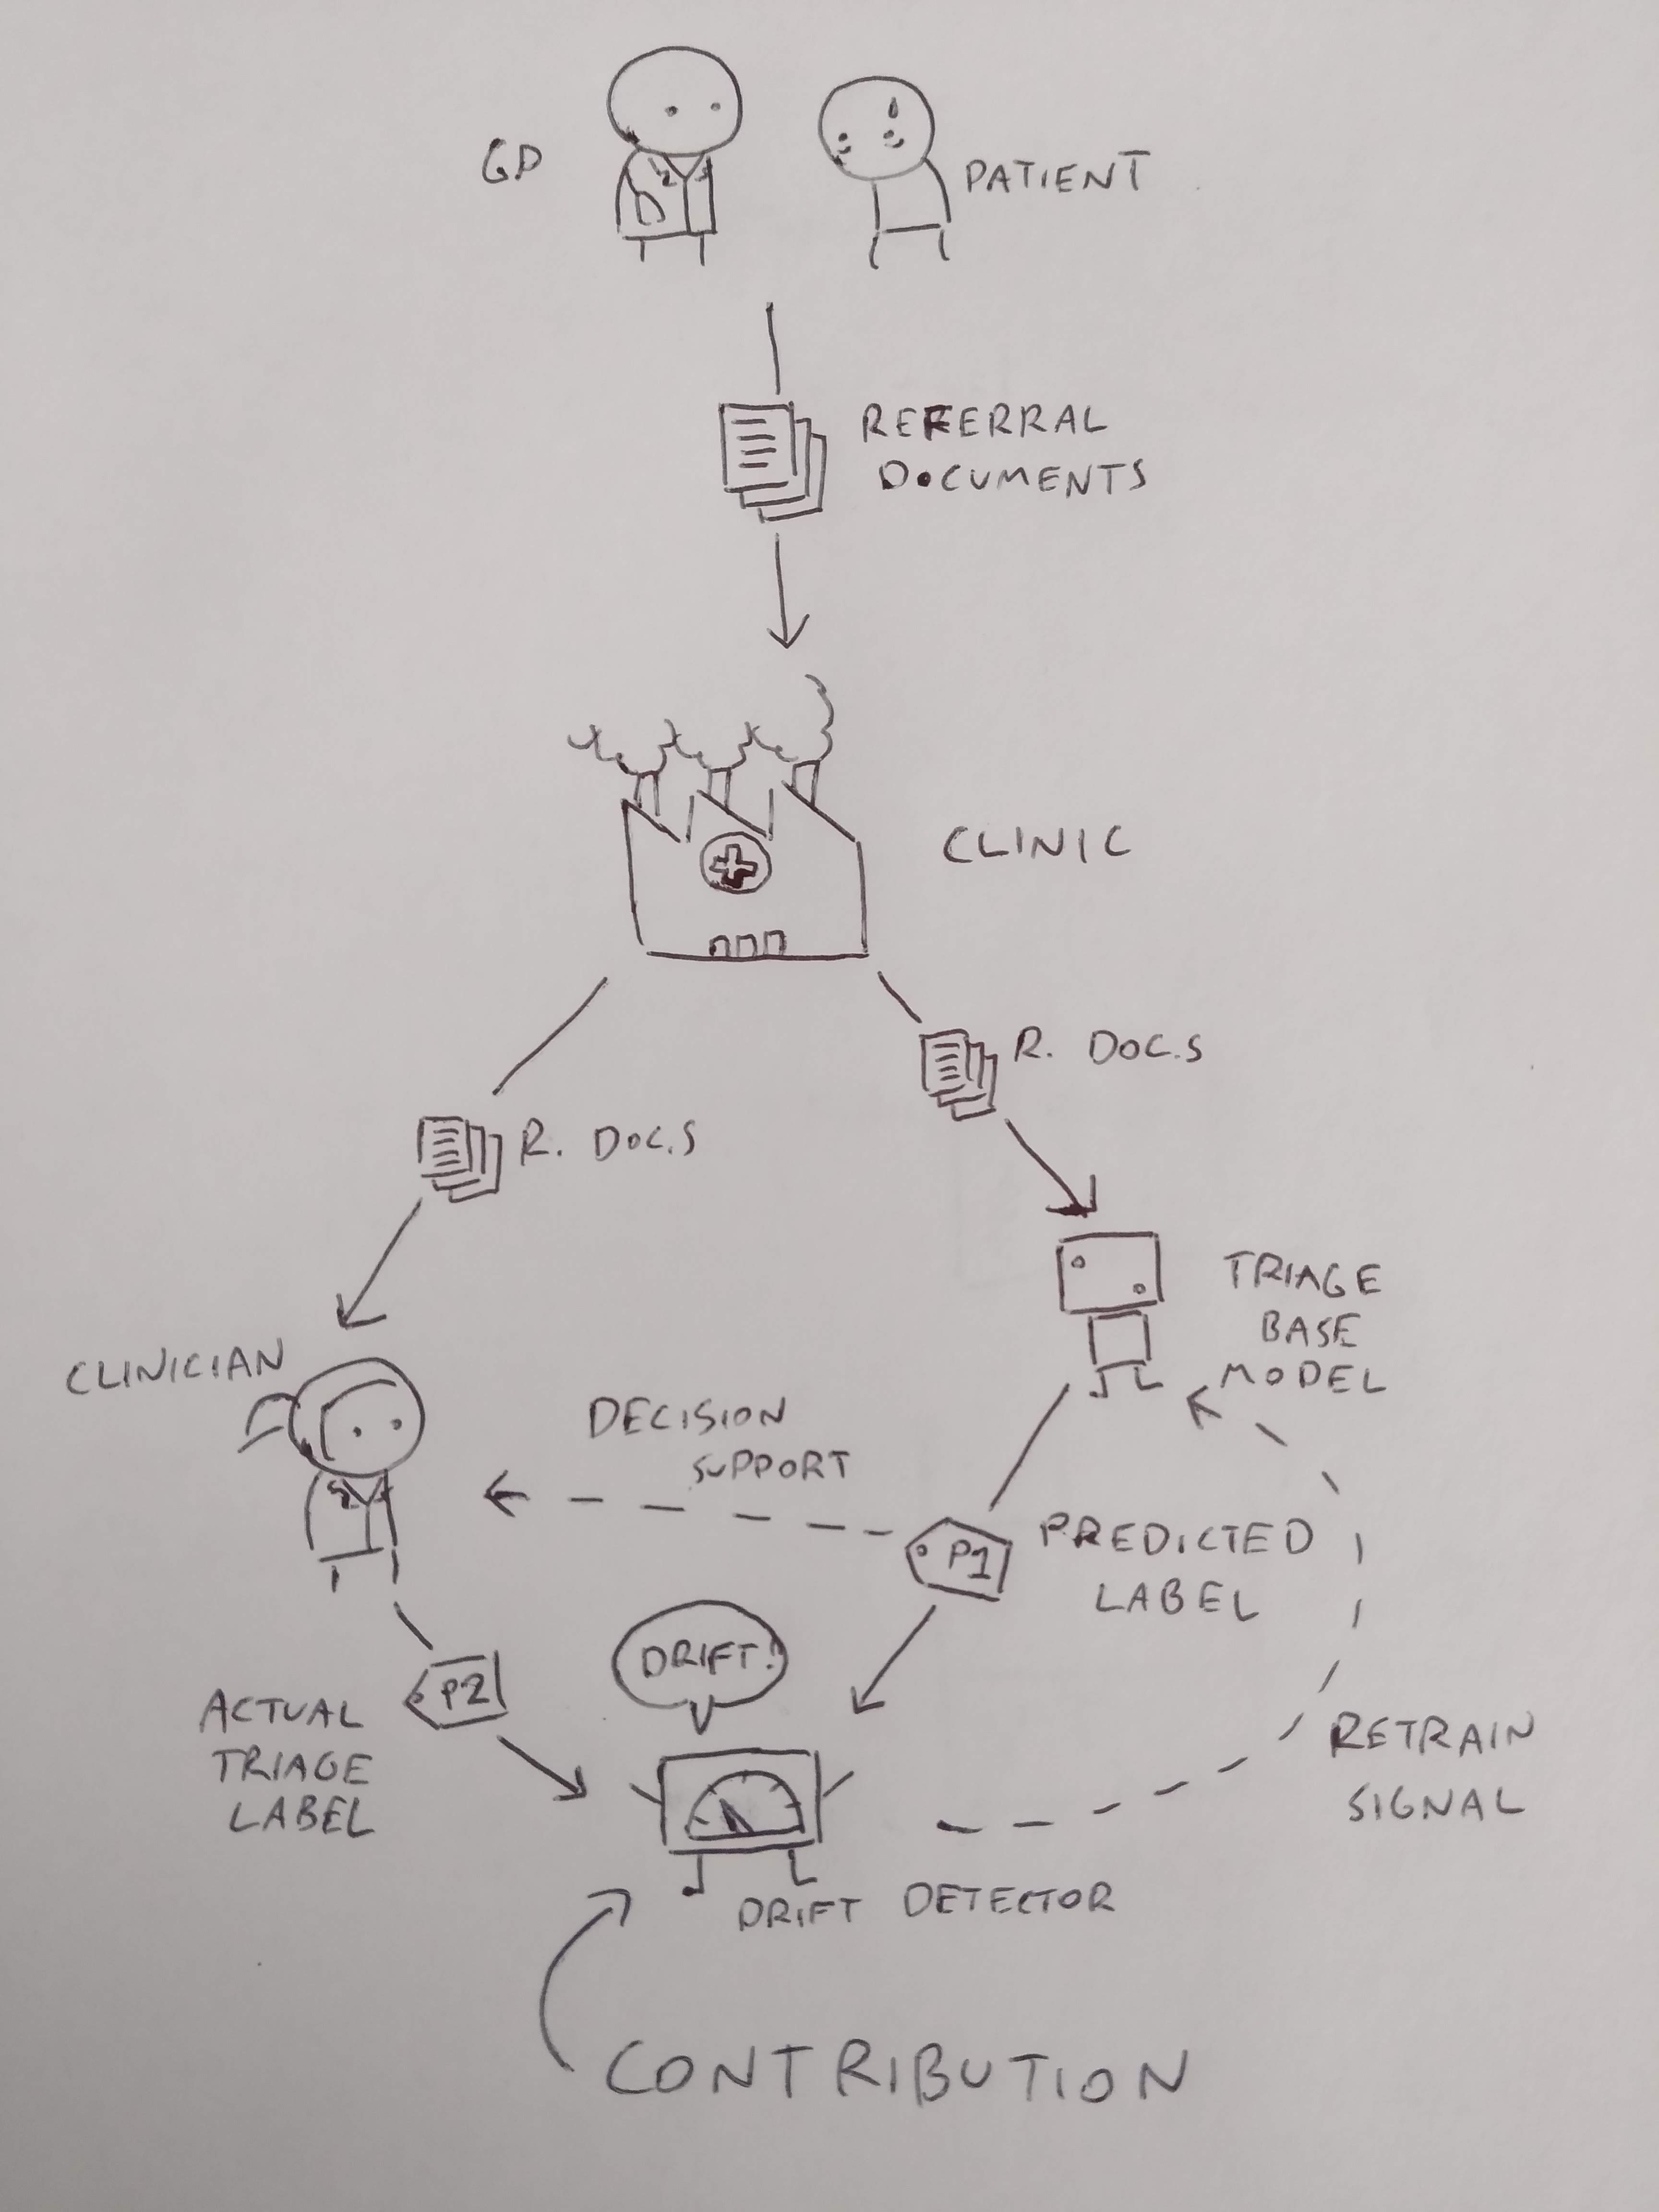
\includegraphics[width=\textwidth]{images/thesis_contribution_illustration.jpg}
%     \caption{The contribution of this thesis.}
%     \label{fig:contribution_illustration}
% \end{figure}

% \section{Structure of this Thesis}

% \begin{itemize}
%     \item Chapter \ref{chapt:Background} provides background on machine learning, data streams, and concept drift detection. 
%     \item Chapter \ref{chapt:MDD} introduces multiple drift detector, a framework for drift detection in practical data science applications. 
%     \item Chapter \ref{chapt:CDDM} introduces calibrated drift detection method (CDDM), a drift detection method which makes use of probabilistic predictions to reduce false positives and false negatives. 
%     \item Chapter \ref{chapt:BDD} introduces bayesian drift detection method (BDDM), a method for exactly calculating posterior probabilities of drift,  and beta with adaptive forgetfulness (BWAF), an efficient heuristic-based drift detection method inspired by BDDM. 
%     \item Chapter \ref{chatp:Experiments} describes three suites of experiments on drift detection methods, both existing methods and our own novel methods, including standard benchmarks and a synthetic GP referrals triage data. 
%     \item Chapter \ref{chapt:Conclusion} concludes this thesis by summarising the key points and discussing directions for future research.
% \end{itemize}